%[a4paper]


\documentclass{article}
%%%%%%%%%%%%%%%%%%%%%%%%%%%%%%%%%%%%%%%%%%%%%%%%%%%%%%%%%%%%%%%%%%%%%%%%%%%%%%%%%%%%%%%%%%%%%%%%%%%%%%%%%%%%%%%%%%%%%%%%%%%%%%%%%%%%%%%%%%%%%%%%%%%%%%%%%%%%%%%%%%%%%%%%%%%%%%%%%%%%%%%%%%%%%%%%%%%%%%%%%%%%%%%%%%%%%%%%%%%%%%%%%%%%%%%%%%%%%%%%%%%%%%%%%%%%
\usepackage{amsfonts}
\usepackage{amsmath}
\usepackage{fullpage}
\usepackage{graphicx}
\usepackage{subfigure}
\usepackage{color,hyperref,cite}

\setcounter{MaxMatrixCols}{10}
%TCIDATA{OutputFilter=LATEX.DLL}
%TCIDATA{Version=5.50.0.2890}
%TCIDATA{<META NAME="SaveForMode" CONTENT="1">}
%TCIDATA{BibliographyScheme=BibTeX}
%TCIDATA{Created=Monday, September 27, 2010 21:32:20}
%TCIDATA{LastRevised=Monday, January 09, 2023 13:19:17}
%TCIDATA{<META NAME="GraphicsSave" CONTENT="32">}
%TCIDATA{<META NAME="DocumentShell" CONTENT="Standard LaTeX\Blank - Standard LaTeX Article">}
%TCIDATA{Language=American English}
%TCIDATA{CSTFile=40 LaTeX article.cst}

\sloppy
\newtheorem{theorem}{Theorem}
\newtheorem{acknowledgement}{Acknowledgement}
\newtheorem{algorithm}{Algorithm}
\newtheorem{axiom}{Axiom}
\newtheorem{case}{Case}
\newtheorem{claim}{Claim}
\newtheorem{conclusion}{Conclusion}
\newtheorem{condition}{Condition}
\newtheorem{conjecture}{Conjecture}
\newtheorem{corollary}{Corollary}
\newtheorem{criterion}{Criterion}
\newtheorem{definition}{Definition}
\newtheorem{observation}{Observation}
\newtheorem{example}{Example}
\newtheorem{exercise}{Exercise}
\newtheorem{lemma}{Lemma}
\newtheorem{notation}{Notation}
\newtheorem{researchproblem}{Research Problem}
\newtheorem{proposition}{Proposition}
\newtheorem{remark}{Remark}
\newtheorem{solution}{Solution}
\newtheorem{summary}{Summary}
\newtheorem{assumption}{Assumption}
\newenvironment{proof}[1][Proof]{\noindent\textbf{#1.} }{\ \rule{0.5em}{0.5em}}
\newenvironment{proofofclaim}[1][Proof]{\noindent\textbf{#1.} }{\ensuremath{\square}}


\begin{document}


\begin{remark}
In the following, we only consider \emph{wasteless} temporal paths. A
temporal path $P=((e_{1},t_{1}),\ldots ,(e_{k},t_{k}))$ is \emph{wasteless}
if, for every $i=1,2,\ldots ,k-1$, we have that $t_{i+1}$ is the first time
after $t_{i}$ that the edge $e_{i+1}$ appears.
\end{remark}

\begin{definition}
\label{arrival-duration-def}Let $u,v\in V$, and let $t\in 
%TCIMACRO{\U{2115} }%
%BeginExpansion
\mathbb{N}
%EndExpansion
$. Given that a temporal path starts within the period $[t,t+\Delta -1]$,
the \emph{arrival} of the fastest path in $(G,\lambda )$ from $u$ to $v$ is $%
A_{t}(u,v)$, and the \emph{arrival} along path $P$ in $(G,\lambda )$ from $u$
to $v$ is $A_{t}(P,u,v)$. Similarly, the \emph{duration} of the fastest path
(resp. the \emph{duration} along path $P$) in $(G,\lambda )$ from $u$ to $v$
is $D(u,v)$ (resp. $D(P,u,v)$).
\end{definition}

Whenever $t=1$, we may omit the index $t$, i.e. we may write $%
A(P,u,v)=A_{1}(P,u,v)$ and $A(u,v)=A_{1}(u,v)$. The following refers to
Figure~\ref{conj-fig}.

Initial assumptions:

\begin{enumerate}
\item $D(u_{0},u_{i})=D(P,u_{0},u_{i})\leq D(Q,u_{0},u_{i})$; denote $\delta
_{0}=D(Q,u_{0},u_{i})-D(u_{0},u_{i})\geq 0$.

\item $D(u_{0},u_{k})=D(Q\cup R,u_{0},u_{k})\leq D(P\cup R,u_{0},u_{k})$.
\end{enumerate}

General properties:

\begin{itemize}
\item $A_{t}(P,u,v)=t_{0}+D(P,u,v)-1$, for every $u,v$, where $t_{0}\in
\lbrack t,t+\Delta -1]$ is the label of the first edge of the path $P$ from $%
u$ to $v$.
\end{itemize}

\bigskip

Let $t_{u_{1}}\in \lbrack 1,\Delta ]$ be the label of the edge $u_{0}u_{1}$,
and denote by $t_{v_{1}}$ the appearance of the edge $u_{0}v_{1}$ within the
period $[t_{u_{1}},t_{u_{1}}+\Delta -1]$. Note that $1\leq t_{u_{1}}\leq
\Delta $ and that $t_{u_{1}}\leq t_{v_{1}}\leq 2\Delta $. By the first
initial assumption, we have:

\begin{equation*}
\delta
_{0}=D(Q,u_{0},u_{i})-D(u_{0},u_{i})=A_{t_{u_{1}}}(Q,u_{0},u_{i})-A_{t_{u_{1}}}(P,u_{0},u_{i})+\left( t_{v_{1}}-t_{u_{1}}\right)
\end{equation*}%
and thus%
\begin{equation}
A_{t_{u_{1}}}(P,u_{0},u_{i})-A_{t_{u_{1}}}(Q,u_{0},u_{i})=t_{v_{1}}-(t_{u_{1}}+\delta _{0})
\label{basic-eq-1}
\end{equation}

\begin{lemma}
\label{lem-1}If $t_{v_{1}}\neq t_{u_{1}}$ then $\delta _{0}\leq \Delta -2$
and $t_{v_{1}}\geq t_{u_{1}}+\delta _{0}+1$.
\end{lemma}

\begin{proof}
First assume that $\delta _{0}\geq \Delta -1$. Then, it follows by (\ref%
{basic-eq-1}) that $%
A_{t_{u_{1}}}(P,u_{0},u_{i})-A_{t_{u_{1}}}(Q,u_{0},u_{i})\leq
t_{v_{1}}-t_{u_{1}}-\Delta +1\leq 0$, and thus $A_{t_{u_{1}}}(P,u_{0},u_{i})%
\leq A_{t_{u_{1}}}(Q,u_{0},u_{i})$. Therefore, since we can traverse path $P$
from $u_{0}$ to $u_{i}$ by departing at time $t_{v_{1}}\geq t_{u_{1}}+1$ and
by arriving no later than traversing path $Q$, we have that $D(P\cup
Q,u_{0},u_{k})<D(Q\cup R,u_{0},u_{k})$, which is a contradiction to the
second initial assumption. Therefore $\delta _{0}\leq \Delta -2$.

Now assume that $t_{u_{1}}+1\leq t_{v_{1}}\leq t_{u_{1}}+\delta _{0}$. Then,
it follows by (\ref{basic-eq-1}) that $A_{t_{u_{1}}}(P,u_{0},u_{i})\leq
A_{t_{u_{1}}}(Q,u_{0},u_{i})$ which is, similarly to the previous case, a
contradiction. Therefore $t_{v_{1}}\geq t_{u_{1}}+\delta _{0}+1$.
\end{proof}

\medskip

The next corollary follows immediately from Lemma \ref{lem-1}.


\begin{corollary}
\label{cor-1}If $t_{v_{1}}\neq t_{u_{1}}$ then $1\leq
A_{t_{u_{1}}}(P,u_{0},u_{i})-A_{t_{u_{1}}}(Q,u_{0},u_{i})\leq \Delta
-1-\delta _{0}$.
\end{corollary}

\begin{lemma}
\label{lem-2}$D(P\cup \{u_{i}u_{i-1}\},u_{0},u_{i-1})>D(Q\setminus
\{u_{i}u_{i-1}\},u_{0},u_{i-1})$.
\end{lemma}

\begin{proof}
Let $e\in \lbrack 1,\Delta ]$ be the label of the edge $u_{i-1}u_{i}$, and
let $f\in \lbrack e+1,e+\Delta ]$ be the time of the first appearance of the
edge $u_{i}u_{i+1}$ after time $e$. Let $A_{t_{u_{i}}}(Q,u_{0},u_{i})=x%
\Delta +e$. Then $A_{t_{u_{i}}}(Q\cup
\{u_{i}u_{i+1}\},u_{0},u_{i+1})=x\Delta +f$. Furthermore let $g$ be such
that $A_{t_{u_{i}}}(P,u_{0},u_{i})=x\Delta +g$. 

\emph{Case 1: }$t_{v_{1}}\neq t_{u_{1}}$\emph{.} Then Corollary \ref{cor-1}
implies that $e+1\leq g\leq e+(\Delta -1-\delta _{0})$. Assume that $g<f$.
Then, we can traverse path $P$ from $u_{0}$ to $u_{i}$ by departing at time $%
t_{v_{1}}\geq t_{u_{1}}+1$ and by arriving at most at time $x\Delta +f-1$,
and thus $D(P\cup R,u_{0},u_{k})<D(Q\cup R,u_{0},u_{k})$, which is a
contradiction to the second initial assumption. Therefore $g\geq f$. That is,%
\begin{equation}
e+1\leq f\leq g\leq e+(\Delta -1-\delta _{0}).  \label{basic-eq-2}
\end{equation}

Consider the path $P^{\ast }=P\cup \{u_{i}u_{i-1}\}$. Assume that we start
traversing $P^{\ast }$ at time $t_{v_{1}}$. Then we arrive at $u_{i}$ at
time $x\Delta +g$, and we continue by traversing edge $u_{i}u_{i-1}$ at time 
$(x+1)\Delta +e$. That is, $D(P^{\ast },u_{0},u_{i-1})=(x+1)\Delta
+e-t_{v_{1}}+1$. 

Now consider the path $Q^{\ast }=Q\setminus \{u_{i}u_{i-1}\}$. Let $h\in
\lbrack 1,\Delta ]$ be such that $A_{t_{u_{i}}}(Q^{\ast
},u_{0},u_{i-1})=x\Delta +e-h$. That is, if we start traversing $Q^{\ast }$
at time $t_{u_{1}}$, we arrive at $u_{i-1}$ at time $x\Delta +e-h$, i.e. $%
D(Q^{\ast },u_{0},u_{i-1})=x\Delta +e-h-t_{u_{1}}+1$. Summarizing, we have:%
\begin{eqnarray*}
D(P^{\ast },u_{0},u_{i-1})-D(Q^{\ast },u_{0},u_{i-1}) &=&\Delta
+h-(t_{v_{1}}-t_{u_{1}}) \\
&\geq &(\Delta -\delta _{0})+h>0,
\end{eqnarray*}%
which proves the statement of the lemma.

\emph{Case 2: }$t_{v_{1}}=t_{u_{1}}$\emph{.} Then, it follows by (\ref%
{basic-eq-1}) that $%
A_{t_{u_{1}}}(P,u_{0},u_{i})=A_{t_{u_{1}}}(Q,u_{0},u_{i})-\delta _{0}\leq
A_{t_{u_{1}}}(Q,u_{0},u_{i})$. Therefore $g\leq e$. Similarly to Case 1
above, consider the paths $P^{\ast }=P\cup \{u_{i}u_{i-1}\}$ and $Q^{\ast
}=Q\setminus \{u_{i}u_{i-1}\}$. Assume that we start traversing $P^{\ast }$
at time $t_{v_{1}}=t_{u_{1}}$. Then we arrive at $u_{i}$ at time $x\Delta +g$%
, and we continue by traversing edge $u_{i}u_{i-1}$, either at time $%
(x+1)\Delta +e$ (in the case where $g=e$) or at time $x\Delta +e$ (in the
case where $g\neq e$). That is, $D(P^{\ast },u_{0},u_{i-1})\geq x\Delta
+e-t_{u_{1}}+1$.

Similarly to Case 1, let $h\in \lbrack 1,\Delta ]$ be such that $%
A_{t_{u_{i}}}(Q^{\ast },u_{0},u_{i-1})=x\Delta +e-h$. That is, if we start
traversing $Q^{\ast }$ at time $t_{u_{1}}$, we arrive at $u_{i-1}$ at time $%
x\Delta +e-h$, i.e. $D(Q^{\ast },u_{0},u_{i-1})=x\Delta +e-h-t_{u_{1}}+1$.
Summarizing, we have:%
\begin{equation*}
D(P^{\ast },u_{0},u_{i-1})-D(Q^{\ast },u_{0},u_{i-1})\geq h\geq 1,
\end{equation*}%
which proves the statement of the lemma.
\end{proof}

\medskip

\begin{figure}[htbp]
\centering
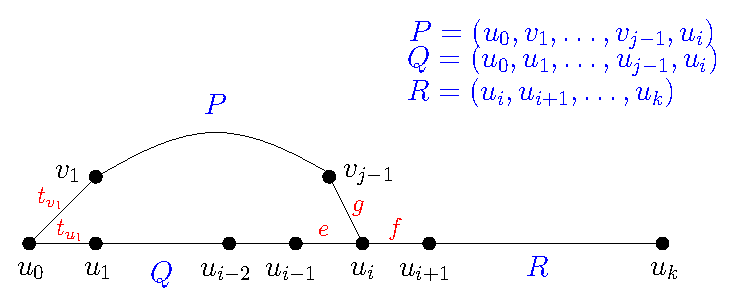
\includegraphics[width=0.6\linewidth]{conj-fig}
\caption{Figure of the conjecture.}
\label{conj-fig}
\end{figure}

%
%
%{\small 
%\bibliographystyle{abbrv}
%\bibliography{ref-evolution}
%}

\end{document}
